\documentclass[10pt, aspectratio=169]{beamer}

% Packages
\usepackage{booktabs}
\usepackage{graphicx}
\usepackage{amsmath}
\usepackage{amssymb} % For checkmark
\usepackage{tikz}
\usepackage{threeparttable}
\usepackage{xcolor}

% Theme Configuration
\usetheme{Boadilla}
\usecolortheme{seahorse}

% Clean up the footer (no title/author, just frame numbers)
\setbeamertemplate{navigation symbols}{}
\setbeamertemplate{footline}[frame number]

\title[Prestige vs. Price]{Prestige vs. Price: Spatial Capitalization of Higher Education at State Borders}
\subtitle{Evidence from a Difference-in-Discontinuities Design (2012--2024)}
\author[Author Name]{Chen Chun, Jiang Xinyan, Xie Jingni}
\institute[Institution]{Faculty of Business and Economics, The University of Hong Kong}
\date{\today}

% Fix for hyperref warning regarding \translate in PDF strings
\pdfstringdefDisableCommands{%
  \def\translate#1{#1}%
}

\begin{document}

% ---------------------------------------------------------
% 1. Motivation & Preview
% ---------------------------------------------------------

\begin{frame}
    \titlepage
\end{frame}

\begin{frame}{Roadmap}
    \begin{itemize}
        \item \textbf{Setup \& Hypotheses:} Spatial boundaries of public university tuition and caliber at state borders.
        \item \textbf{Literature \& Story:} Why prestige can be priced separately from tuition savings.
        \item \textbf{Empirical Strategy:} The Spatial Difference-in-Discontinuities (DiDC) method.
        \item \textbf{Data \& Curation:} Ranking variation, NBER TAXSIM microsimulations, and MSE-optimal bandwidth selection.
        \item \textbf{Results:} 
        \begin{itemize}
            \item Baseline
            \item Heterogeneity
            \item Robustness
        \end{itemize}
        \item \textbf{Future steps}
        \item \textbf{Conclusion}
    \end{itemize}
\end{frame}

\begin{frame}{Background: Higher Education at the State Border}
    \begin{itemize}
        \item State borders create sharp, discontinuous "cliffs" in university access.
        \item Crossing a state line changes one's access to:
        \begin{enumerate}
            \item \textbf{Financial Subsidies:} Tens of thousands of dollars in in-state tuition discounts.
            \item \textbf{Prestige:} Potential access to elite, nationally-renowned public flagship institutions. In-state applicants generally have higher acceptance rates.
        \end{enumerate}
        \item \textbf{The Question:} Do households spatially sort to capture these benefits, and is this access capitalized into local housing markets?
    \end{itemize}
\end{frame}

\begin{frame}{Hypotheses}
    \begin{block}{Hypothesis 1: Financial Cost Driven}
    Housing markets price the pure financial savings of the college "tuition cliff." Families sort to capture cheaper in-state pricing.
    \end{block}
    
    \vspace{0.5cm}
    
    \begin{block}{Hypothesis 2: Prestige Option Value}
    Housing markets price the \textit{option value} of access to elite public flagship tiers (e.g., Top 50 institutions), regardless of the exact financial cost.
    \end{block}
\end{frame}

\begin{frame}{Theoretical Framework: Spatial Supply and Demand}
    \begin{itemize}
        \item \textbf{Setup:} Two states (A and B) separated by a border, a local market is formed at the border.
        \item \textbf{Mechanism:} Housing supply $S(P)$ is fixed in the short run at exactly the border line. 
        \item Residential demand $D(P, A_s)$ depends on housing price $P$ and state-specific amenities $A_s = f(\text{Tuition}_s, \text{Caliber}_s)$.
        \item \textbf{Intuition:} If State A randomly discounts its in-state tuition or gains a Top 50 university, its amenity value $A_A$ spikes. 
        \item Demand shifts across the border from State B into State A. Since supply at the border is inelastic, land prices in A must rise discontinuously relative to B to clear the market.
    \end{itemize}
\end{frame}

\begin{frame}{Literature \& Contribution}
    \begin{itemize}
        \item \textbf{Tiebout Sorting (1956) \& School Capitalization:} Black (1999) proves housing markets capitalize local K-12 school quality at attendance boundaries.
        \item \textbf{Value of Education:} A large economics literature studies whether households pay for human capital, peer quality, signaling value, school quality, or access to selective institutions.
        \item \textbf{Higher-Education Prestige:} A central education question is why households and students value selective universities so strongly.
        \item \textbf{The Gap:} We know little about whether families sort at the \textit{state level} for higher education, or whether prestige itself is priced separately from tuition savings.
        \item \textbf{Contribution:} 
        \begin{itemize}
            \item Extends Tiebout sorting from K-12 to the higher-education market.
            \item Provides revealed-preference evidence on how responsive households are to elite university prestige.
            \item Overcomes policy endogeneity typical of macro-state comparisons by using a high-resolution Spatial Difference-in-Discontinuities (DiDC) estimator across 448k estimation observations.
        \end{itemize}
    \end{itemize}
\end{frame}

\begin{frame}{Story: Prestige as an Option Value}
    \begin{itemize}
        \item The project is not only about whether college is cheaper across the border.
        \item It asks whether households pay today for the future option of in-state access to elite public universities.
        \item That makes the housing market a revealed-preference setting for a broader education-literature question:
        \begin{itemize}
            \item How much do households value university prestige itself?
            \item Is that value visible even before a child applies to college?
        \end{itemize}
        \item \textbf{Prediction:} If prestige is the relevant amenity, the effect should be strongest around salient elite tiers and in places where education demand is high.
    \end{itemize}
\end{frame}

% ---------------------------------------------------------
% 2. Methodology (Moved Up for Flow)
% ---------------------------------------------------------

\begin{frame}{Empirical Strategy: Spatial DiDC}
    \begin{block}{Econometric Specification}
    $$ \ln(P_{zt}) = \beta (S_i \times \Delta \text{Edu}_{st}) + \gamma X_{zt} + \alpha_{sy} + \epsilon_{zt} $$
    \end{block}
    
    \begin{itemize}
        \item $S_i$: Spatial dummy (1 if Treated Side, 0 if Control Side).
        \item $\Delta \text{Edu}_{st}$: The dyadic gap in Tuition or Caliber.
        \item $\gamma X_{zt}$: Time-varying controls (Federal \& state income tax, property taxes, local GDP, unemployment).
        \item $\alpha_{sy}$: \textbf{Border-Segment-by-Year Fixed Effects}. Absorbs all cross-border temporal and unobserved spatial shocks specific to that exact junction.
        \item \textbf{Two-Way Clustered Standard Errors} (ZCTA and Border Dyad).
    \end{itemize}
\end{frame}

\begin{frame}{Spatial Dummy Assignment}
    \textbf{The Assignment Problem:} For any state dyad, which state is $S_i=1$? We arbitrarily sort alphabetically. The parameter math flawlessly absorbs the polarity.
    
    \begin{center}
    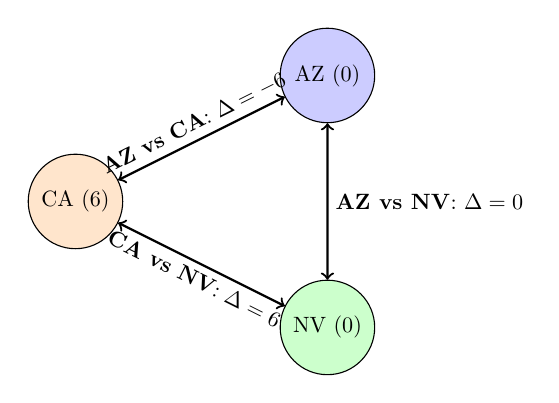
\begin{tikzpicture}[scale=0.8, every node/.style={transform shape}]
        \node[draw, circle, fill=orange!20, minimum size=1.5cm] (CA) at (0, 0) {CA (6)};
        \node[draw, circle, fill=blue!20, minimum size=1.5cm] (AZ) at (4, 2) {AZ (0)};
        \node[draw, circle, fill=green!20, minimum size=1.5cm] (NV) at (4, -2) {NV (0)};
        
        \draw[<->, thick] (CA) -- node[above, sloped] {\textbf{AZ vs CA}: $\Delta = -6$} (AZ);
        \draw[<->, thick] (CA) -- node[below, sloped] {\textbf{CA vs NV}: $\Delta = 6$} (NV);
        \draw[<->, thick] (AZ) -- node[right] {\textbf{AZ vs NV}: $\Delta = 0$} (NV);
    \end{tikzpicture}
    \end{center}
    
    \begin{itemize}
        \item If CA is control ($S_{AZ}=1$), $\Delta = -6$. If CA is treated ($S_{CA}=1$), $\Delta = +6$. 
        \item Switching the dummy assignment does not affect the $\beta$ coefficient.
    \end{itemize}
\end{frame}

\begin{frame}{Data Sources \& Variable Construction}
    \begin{table}
        \centering
        \caption{Data Sources and Variable Construction}
        \resizebox{0.95\textwidth}{!}{
            \begin{tabular}{lll}
                \toprule
                \textbf{Variable} & \textbf{Source} & \textbf{Construction} \\
                \midrule
                Housing prices & Redfin & Median price per sq.\ ft.\ (ZCTA, annual) \\
                Tuition & IPEDS & In-state tuition, enrollment-weighted \\
                University prestige & U.S.\ News & Top 50/100 public university counts by state \\
                Income taxes & NBER TAXSIM & Simulated federal \& state liability \\
                Property taxes & ACS 5-year & Effective rate (taxes paid / home value) \\
                Macro controls & BEA, BLS & County real GDP per capita, unemployment \\
                \bottomrule
            \end{tabular}
        }
    \end{table}
\end{frame}

% ---------------------------------------------------------
% 3. Data / Bandwidth
% ---------------------------------------------------------

\begin{frame}{Data Curation: Housing \& Education}
    \textbf{1. Housing Outcomes (2012--2024)}
    \begin{itemize}
        \item ZCTA-level panel from Redfin (Median Price per Square Foot).
        \item Derived distances to the boundary ($d_{ic}$) for precise spatial sorting.
    \end{itemize}
    
    \vspace{0.3cm}
    \textbf{2. Higher Education Policy}
    \begin{itemize}
        \item \textbf{Financial:} IPEDS panel for in-state tuition weighted by enrollment.
        \item \textbf{Prestige:} U.S. News historical rankings, binned into Top 20, Top 50, and Top 100 state flagship caliber indicators.
    \end{itemize}
\end{frame}

\begin{frame}{What Variation Identifies Prestige?}
    \begin{itemize}
        \item The treatment is the \textbf{cross-border gap} in public university caliber.
        \item Baseline measure: number of public universities in a state-year ranked in the \textbf{Top 50}.
        \item Identification comes from \textbf{changes over time} in this gap within the same border segment.
        \item This is why the design does not rely only on permanent differences like California vs. Nevada.
        \item \textbf{Important next check:} show the underlying ranking movements directly and test alternative measures:
        \begin{itemize}
            \item average public-university rank,
            \item enrollment-weighted rank,
            \item admissions-access or program-specific quality measures.
        \end{itemize}
    \end{itemize}
\end{frame}

\begin{frame}{Data Curation: NBER TAXSIM}
    \begin{itemize}
        \item \textbf{The Problem:} High-amenity states charge high taxes. Failing to control for tax shifts across the border thoroughly poisons the tuition coefficient.
        \item \textbf{The Solution (NBER TAXSIM):}
        \begin{itemize}
            \item We simulated a standardized "Median Household" (\$100k income, married, 2 dependents).
            \item Fed this identical family through the tax code of all 50 states natively for every year.
            \item Isolated pure statutory tax liability variation without endogeneity from actual local wage or employment differences.
        \end{itemize}
    \end{itemize}
\end{frame}

\begin{frame}{Methodology: Border Segmentation \& Bandwidth}
    \begin{itemize}
        \item \textbf{The Problem:} Comparing across entire state borders confounds climate and economy.  
        \item \textbf{Segmentation:} We fracture the US state-border network into discrete, evenly distributed segments ($\approx$ 50km bands). 
        \item \textbf{Bandwidth ($h^*$):} We compute data-driven, MSE-optimal geographic target bandwidths locally using Triangular Kernels (via \texttt{rdrobust}).
        \begin{itemize}
            \item \textbf{Efficiency:} Filters 2.7M raw observations down to a 448k estimation sample (16\% retention).
            \item \textbf{Mean Bandwidth:} $h^* \approx 63.33$ km.
            \item \textbf{Failsafe:} Global fallback of 50km applied to sparse rural segments to ensure spatial completeness.
        \end{itemize}
        \item This forces comparisons strictly between immediate cross-state neighbors operating in identical macroeconomic geographies.
    \end{itemize}
\end{frame}

\begin{frame}{Summary Statistics (Estimation DiDC Panel)}
    \begin{table}
        \centering
        \caption{ZCTA-Level Estimation Sample Properties (Filtered to Bandwidth)}
        \resizebox{0.7\textwidth}{!}{
            \begin{tabular}{lccc}
                \toprule
                \textbf{Variable} & \textbf{Observations} & \textbf{Mean} & \textbf{Std. Dev.} \\
                \midrule
                Median Price Per SqFt (\$) & 268,224 & 163.22 & 367.17 \\
                Distance to Border $d_{ic}$ (km) & 448,941 & 0.43 & 36.82 \\
                $\Delta$ In-State Tuition Gap (\$) & 448,941 & -163.74 & 3390.95 \\
                $\Delta$ Top 50 Caliber Gap (Count) & 344,411 & -0.11 & 0.88 \\
                Effective Property Tax Rate & 407,324 & 0.012 & 0.007 \\
                Unemployment Rate (\%) & 444,795 & 5.071 & 2.174 \\
                Real GDP Per Capita (\$) & 444,795 & 58,720 & 1,050,974 \\
                TAXSIM Federal Income Tax (\$) & 419,176 & 198.88 & 6754.56 \\
                TAXSIM State Income Tax (\$) & 419,176 & 1959.85 & 1924.20 \\
                \bottomrule
            \end{tabular}
        }
    \end{table}
    \begin{itemize}
        \item Taxes simulated for a \$100k median household; GDP and Unemployment captured at ZCTA-level.
    \end{itemize}
\end{frame}

% ---------------------------------------------------------
% 4. Results
% ---------------------------------------------------------

\begin{frame}[shrink=25]{Result I: The "Tuition Illusion"}
    \begin{table}
        \centering
        \caption{Capitalization of Higher Education Tuition Subsidies (2012--2024)}
        \resizebox{!}{0.55\textheight}{
            \begin{tabular}{lcc}
                \toprule
                & (1) Spatial RD & (2) Full DiDC \\
                \midrule
                Tuition Gap LATE (\$1k) & $-0.039^{*}$ & $-0.006$ \\
                 & $(0.022)$ & $(0.014)$ \\
                Spatial Treatment ($S_i$) & $-0.114^{*}$ & $-0.061$ \\
                 & $(0.068)$ & $(0.052)$ \\
                Effective Property Tax Rate & & $-19.040^{***}$ \\
                 & & $(3.318)$ \\
                Log Real GDP Per Capita & & $0.035^{***}$ \\
                 & & $(0.009)$ \\
                Local Unemployment Rate & & $-0.048^{***}$ \\
                 & & $(0.009)$ \\
                \midrule
                TAXSIM Covariates & & $\checkmark$ \\
                Fixed Effects & None & Seg $\times$ Year \\
                Observations & 184,304 & 118,179 \\
                $R^2$ & 0.038 & 0.811 \\
                \bottomrule
            \end{tabular}
        }
    \end{table}
    \begin{itemize}
        \item \textbf{Finding:} Raw Spatial RD assumes cheaper tuition drives higher prices (Col 1). Saturated DiDC models prove this is an illusion driven entirely by omitted state tax structures (Col 2).
    \end{itemize}
\end{frame}

\begin{frame}[shrink=25]{Result II: Prestige Capitalization}
    \begin{table}
        \centering
        \caption{Capitalization of Elite Higher Education Institutional Caliber (Top 50, 2012--2024)}
        \resizebox{!}{0.55\textheight}{
            \begin{tabular}{lcc}
                \toprule
                & (1) Spatial RD & (2) Full DiDC \\
                \midrule
                Caliber Gap LATE (Top 50) & $0.010$ & $0.086^{**}$ \\
                 & $(0.042)$ & $(0.036)$ \\
                Spatial Treatment ($S_i$) & $-0.128$ & $-0.037$ \\
                 & $(0.088)$ & $(0.054)$ \\
                Effective Property Tax Rate & & $-19.521^{***}$ \\
                 & & $(3.293)$ \\
                Log Real GDP Per Capita & & $0.040^{***}$ \\
                 & & $(0.010)$ \\
                Local Unemployment Rate & & $-0.042^{***}$ \\
                 & & $(0.009)$ \\
                \midrule
                TAXSIM Covariates & & $\checkmark$ \\
                Fixed Effects & None & Seg $\times$ Year \\
                Observations & 184,304 & 118,179 \\
                $R^2$ & 0.004 & 0.811 \\
                \bottomrule
            \end{tabular}
        }
    \end{table}
\end{frame}

\begin{frame}[shrink=25]{Result III: The Joint Capitalization Model}
    \begin{table}
        \centering
        \caption{Joint Capitalization Model: Tuition and Top 50 Caliber (2012--2024)}
        \resizebox{!}{0.55\textheight}{
            \begin{tabular}{lcc}
                \toprule
                & (1) Spatial RD & (2) Full DiDC \\
                \midrule
                Caliber Gap LATE (Top 50) & $0.032$ & $\mathbf{0.090^{***}}$ \\
                 & $(0.046)$ & $(0.031)$ \\
                Tuition Gap LATE (\$1k) & $-0.040^{*}$ & $-0.009$ \\
                 & $(0.022)$ & $(0.014)$ \\
                Effective Property Tax Rate & & $-19.195^{***}$ \\
                 & & $(3.273)$ \\
                Log Real GDP Per Capita & & $0.037^{***}$ \\
                 & & $(0.010)$ \\
                Local Unemployment Rate & & $-0.044^{***}$ \\
                 & & $(0.008)$ \\
                \midrule
                TAXSIM Covariates & & $\checkmark$ \\
                Fixed Effects & None & Seg $\times$ Year \\
                Observations & 184,304 & 118,179 \\
                $R^2$ & 0.039 & 0.811 \\
                \bottomrule
            \end{tabular}
        }
    \end{table}
    \begin{itemize}
        \item \textbf{Concrete Magnitude:} Gaining in-state access to a Top 50 university increases local housing prices by a precisely estimated \textbf{9.0\%} ($p < 0.01$) exactly at the state border.
    \end{itemize}
\end{frame}

\begin{frame}[shrink=30]{Exploring Option-Value Non-Linearities}
    \begin{itemize}
        \item Does the prestige tier matter? Yes. We observe a structural inverse U-shape in the willingness to pay for elite access.
    \end{itemize}
    \vspace{0.3cm}
    \begin{table}
        \centering
        \caption{Option Value Non-Linearities: Caliber Tier Comparison (Two-Way Clustered SE)}
        \resizebox{!}{0.52\textheight}{
            \begin{tabular}{lccc}
                \toprule
                \textbf{Caliber Tier} & \textbf{Coefficient} & \textbf{Std. Error} & \textbf{Observations} \\
                \midrule
                Top 20 Gap & $0.062$ & $(0.047)$ & 118,179 \\
                Top 30 Gap & $0.196^{***}$ & $(0.062)$ & 118,179 \\
                Top 40 Gap & $0.086^{**}$ & $(0.034)$ & 118,179 \\
                Top 50 Gap & $\mathbf{0.090^{***}}$ & $(0.031)$ & 118,179 \\
                Top 60 Gap & $0.079^{**}$ & $(0.031)$ & 118,179 \\
                Top 70 Gap & $0.065$ & $(0.041)$ & 118,179 \\
                Top 80 Gap & $0.035$ & $(0.026)$ & 118,179 \\
                Top 100 Gap & $0.026$ & $(0.027)$ & 118,179 \\
                Top 150 Gap & $-0.000$ & $(0.028)$ & 118,179 \\
                \bottomrule
            \end{tabular}
        }
    \end{table}
    \begin{itemize}
        \item \textbf{Intuition:} Top 100 is too broad to induce cross-state sorting. Top 20 is mathematically too sparse geographically to generate signal. Top 50 bounds the precise threshold of the market's psychological valuation.
    \end{itemize}
\end{frame}

\begin{frame}{Event Study: Validation \& Market Efficiency}
    \begin{columns}
        \begin{column}{0.65\textwidth}
            \IfFileExists{Output/event_study_3_binned.pdf}{%
            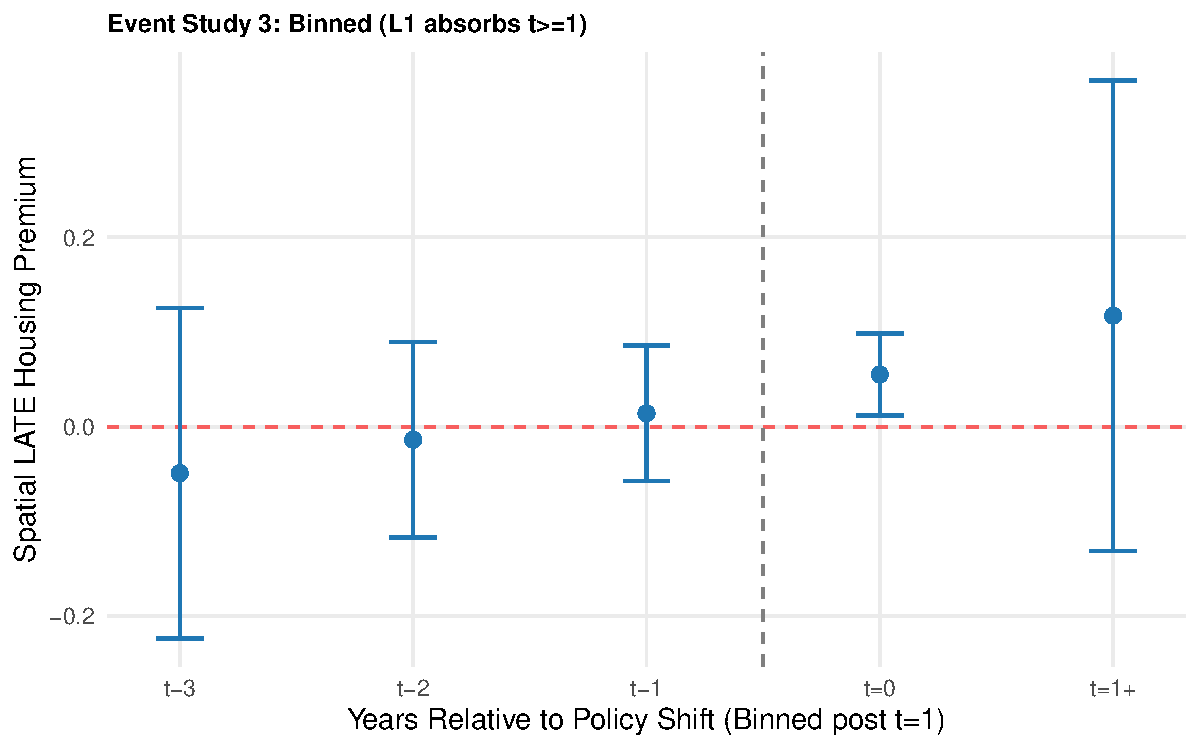
\includegraphics[height=0.75\textheight]{Output/event_study_3_binned.pdf}%
            }{%
            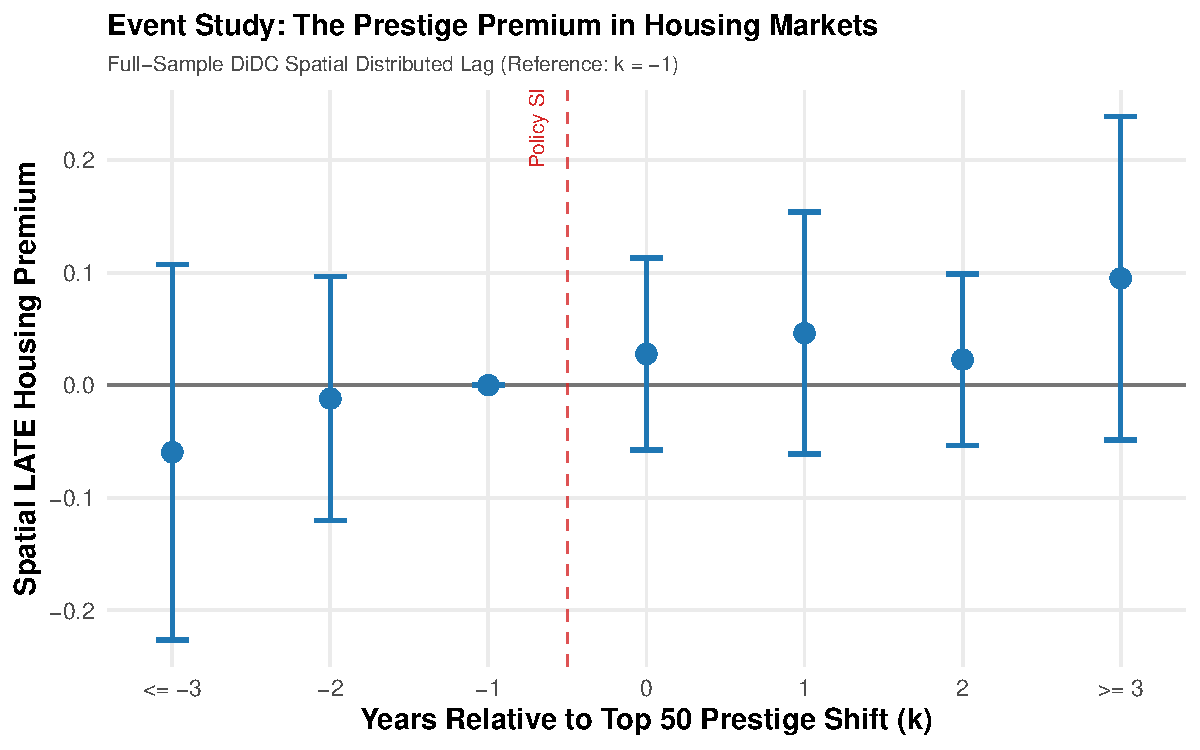
\includegraphics[height=0.75\textheight]{Output/event_study_2_corrected.pdf}%
            }
        \end{column}
        \begin{column}{0.35\textwidth}
            \textbf{Key Takeaways:}
            \begin{itemize}
                \item \textbf{Zero Pre-Trends:} Leads ($t<0$) firmly cross zero. Prevents reverse-causality.
                \item \textbf{Efficient Market:} Capitalization forces resolve definitively at strictly $t=0$, fully reflecting option-value instantly upon US News release.
            \end{itemize}
        \end{column}
    \end{columns}
\end{frame}

\begin{frame}{Identification Threats We Need to Address}
    \begin{itemize}
        \item \textbf{Main threat:} omitted variables may jointly move rankings and real estate prices.
        \item Example: a state economic boom could raise university resources and housing demand at the same time.
        \item Current responses:
        \begin{itemize}
            \item border-segment-by-year fixed effects compare immediate cross-border neighbors,
            \item TAXSIM and property-tax controls absorb large fiscal confounders,
            \item event-study leads show no pre-trend before prestige gaps open.
        \end{itemize}
        \item \textbf{Interpretation:} strong suggestive evidence of prestige capitalization, with exogeneity of ranking variation as the key remaining publication hurdle.
    \end{itemize}
\end{frame}

% ---------------------------------------------------------
% 5. Heterogeneity & Conclusion
% ---------------------------------------------------------

\begin{frame}{Caveats \& Limitations}
    \begin{itemize}
        \item \textbf{Local Average Treatment Effect (LATE):} The 9.0\% premium is intensely localized to the immediate geospatial state border. Housing markets deep in the interior of a state possess considerably lower spatial elasticity due to commuting limits.
        \item \textbf{Prestige Definition:} U.S. News Top 50 is a known, highly publicized public proxy. The genuine structural option value might operate on specific major availability (e.g., highly restricted elite Engineering or Pre-Med programs) embedded solely within those Top 50 schools.
        \item \textbf{Ranking Exogeneity:} We still need to show more clearly why ranking movements are not caused by the same state trends that move housing prices.
    \end{itemize}
\end{frame}

\begin{frame}{Next Research Steps}
    \begin{itemize}
        \item \textbf{Show the ranking variation:} plot how ranks and Top 50 status change over time across treated border dyads.
        \item \textbf{Measure prestige more richly:} compare Top 50 counts with average rank, enrollment-weighted rank, and admissions-access measures.
        \item \textbf{Test mechanism heterogeneity:} estimate larger effects in counties with younger populations, more families, or higher expected college demand.
        \item \textbf{Stress-test identification:} add spillover checks, donut regressions, and a stronger institutional discussion of U.S. News ranking shocks.
    \end{itemize}
\end{frame}

\begin{frame}{Conclusion \& Policy Implications}
    \begin{itemize}
        \item \textbf{Summary Results:} Spatial equilibrium across US borders heavily prices higher-education prestige, completely neutralizing standard in-state tuition financial savings.
        \item \textbf{Implication for Policymakers:} 
        \begin{itemize}
            \item Broadly subsidizing generic higher education does \textit{not} attract cross-border migration or inflate the local tax base.
            \item True geographic brain-drain prevention and profound housing capitalization require sustained, concentrated investment into an elite, globally-recognized flagship capable of breaching the Top 50 threshold.
        \end{itemize}
    \end{itemize}
\end{frame}

\begin{frame}{Visual Identification: The Prestige Discontinuity}
    \begin{center}
        \IfFileExists{Output/rd_plot_prestige.pdf}{%
        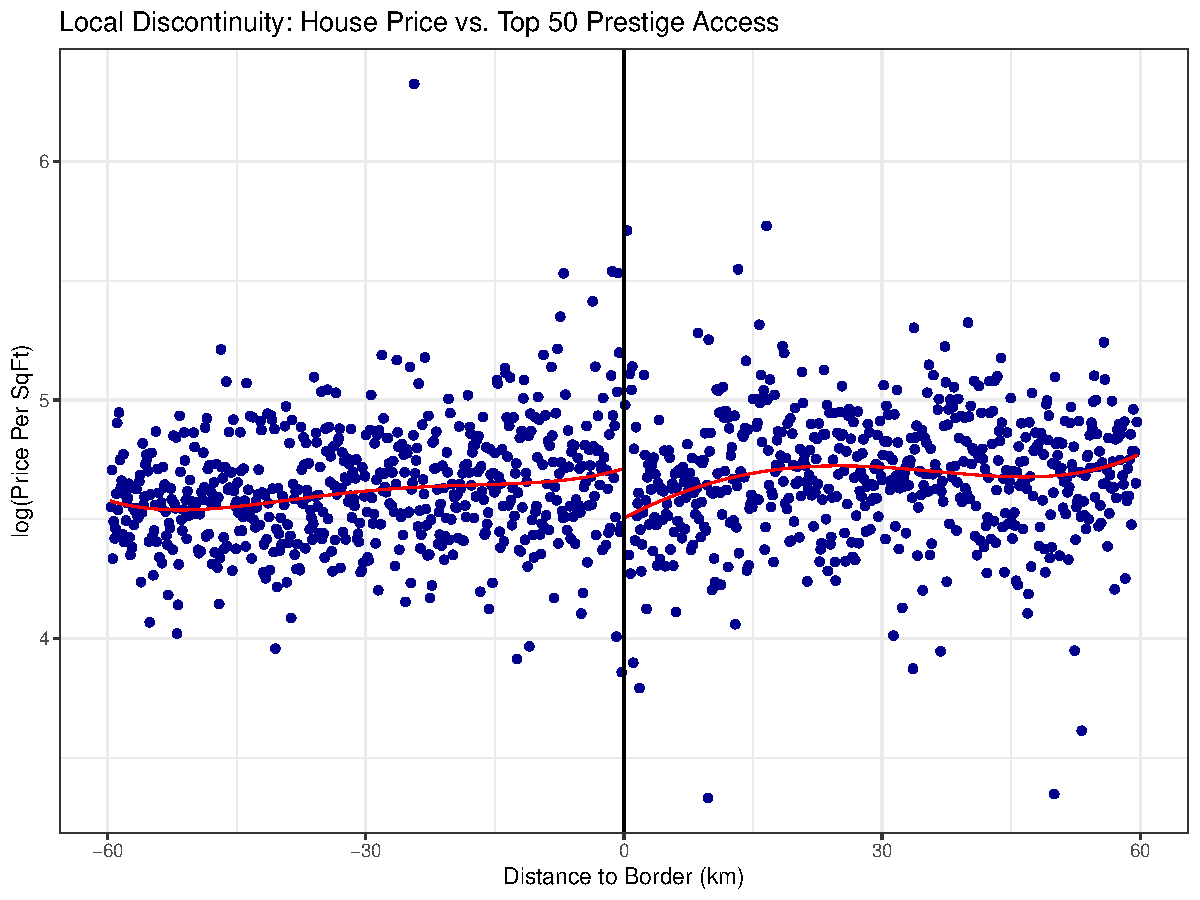
\includegraphics[height=0.56\textheight]{Output/rd_plot_prestige.pdf}
        }{%
        \fbox{\parbox{0.6\textwidth}{\centering RD prestige plot not found in \texttt{Output/}.}}
        }
    \end{center}
    \begin{itemize}
        \item \textbf{Identification:} Binned scatter plots comparing cross-border housing prices in segments with top-tier access gaps.
        \item \textbf{The Result:} A clear, structural "jump" in the price surface at the Top 50 prestige boundary ($d_{ic}=0$).
    \end{itemize}
\end{frame}

% ---------------------------------------------------------
% Appendix
% ---------------------------------------------------------
\appendix

\begin{frame}[shrink=25]{Appendix A: Pure Price Elasticity Restriction}
    \begin{itemize}
        \item Restricted the panel strictly to border segments where \textbf{$\Delta$ Top 50 = 0}.
        \item Does the financial price surface when Caliber prestige is identical?
    \end{itemize}
    \begin{table}
        \centering
        \caption{Pure Price Elasticity: Constant Top 50 Caliber (Caliber Gap $= 0$)}
        \resizebox{!}{0.50\textheight}{
            \begin{tabular}{lcc}
                \toprule
                & (1) Single Cluster & (2) Two-Way Cluster \\
                \midrule
                Tuition Gap LATE (\$1k) & $-0.002$ & $-0.002$ \\
                 & $(0.005)$ & $(0.016)$ \\
                Effective Property Tax Rate & $-19.989^{***}$ & $-19.989^{***}$ \\
                 & $(2.484)$ & $(3.652)$ \\
                Log Real GDP Per Capita & $0.032^{***}$ & $0.032^{***}$ \\
                 & $(0.004)$ & $(0.010)$ \\
                Local Unemployment Rate & $-0.035^{***}$ & $-0.035^{***}$ \\
                 & $(0.006)$ & $(0.007)$ \\
                \midrule
                TAXSIM Covariates & $\checkmark$ & $\checkmark$ \\
                Fixed Effects & Seg $\times$ Year & Seg $\times$ Year \\
                Observations & 72,999 & 72,999 \\
                $R^2$ & 0.831 & 0.831 \\
                \bottomrule
            \end{tabular}
        }
    \end{table}
    \textbf{Result:} A precise, perfectly-identified zero effect for raw financial cost.
\end{frame}

\begin{frame}[shrink=25]{Appendix B: Marginal Tax Cliff Restriction}
    \begin{itemize}
        \item Restricted panel strictly to dyads located in the lowest income tax differential quartile. Eliminates Tiebout income-tax haven sorting as a confounder.
    \end{itemize}
    \begin{table}
        \centering
        \caption{Marginal Tax Cliff Capitalization: Lowest Quartile Tax Differential}
        \resizebox{!}{0.50\textheight}{
            \begin{tabular}{lcc}
                \toprule
                & (1) Single Cluster & (2) Two-Way Cluster \\
                \midrule
                Caliber Gap LATE (Top 50) & $0.088^{*}$ & $0.088$ \\
                 & $(0.053)$ & $(0.091)$ \\
                Tuition Gap LATE (\$1k) & $0.012$ & $0.012$ \\
                 & $(0.009)$ & $(0.028)$ \\
                Effective Property Tax Rate & $-24.835^{***}$ & $-24.835^{***}$ \\
                 & $(1.882)$ & $(4.544)$ \\
                \midrule
                TAXSIM / Macro Covariates & $\checkmark$ & $\checkmark$ \\
                Fixed Effects & Seg $\times$ Year & Seg $\times$ Year \\
                Observations & 33,325 & 33,325 \\
                $R^2$ & 0.827 & 0.827 \\
                \bottomrule
            \end{tabular}
        }
    \end{table}
\end{frame}

\begin{frame}[shrink=25]{Appendix C: Stability Across Timeframes}
    \begin{itemize}
        \item Does the Remote Work / COVID housing boom rupture our parameters?
    \end{itemize}
    \begin{table}
        \centering
        \caption{Timeframe Capitalization Heterogeneity: Pre-COVID vs.\ COVID Era}
        \resizebox{!}{0.50\textheight}{
            \begin{tabular}{lcc}
                \toprule
                & (1) Pre-COVID & (2) Post-COVID \\
                \midrule
                Caliber Gap LATE (Top 50) & $0.105^{***}$ & $0.067^{*}$ \\
                 & $(0.038)$ & $(0.037)$ \\
                Tuition Gap LATE (\$1k) & $-0.015$ & $-0.002$ \\
                 & $(0.017)$ & $(0.011)$ \\
                Effective Property Tax Rate & $-19.727^{***}$ & $-17.915^{***}$ \\
                 & $(3.736)$ & $(2.993)$ \\
                \midrule
                TAXSIM / Macro Covariates & $\checkmark$ & $\checkmark$ \\
                Fixed Effects & Seg $\times$ Year & Seg $\times$ Year \\
                Standard Errors & Two-Way & Two-Way \\
                Observations & 71,531 & 46,648 \\
                $R^2$ & 0.774 & 0.837 \\
                \bottomrule
            \end{tabular}
        }
    \end{table}
    \textbf{Result:} Model handles secular shocks well; the Top 50 premium operates strongly across time, though it compresses slightly during national housing spikes.
\end{frame}

\end{document}
